\begin{frame}
  \frametitle{6.4 (Janvier 2018)}

  \begin{itemize}
  \item Améliorations du widget de sélection des fichiers multiples
  \item Application et filtre pour l'amélioration du contraste local (CLAHE)
  \item Amélioration du modèle générique de capteur SAR
  \item Support de python 3
  \item Après cette release: déménagement vers gitlab!
  \end{itemize}  
\end{frame}

\begin{frame}
  \frametitle{Gitlab: plus facile, plus intégré}
  \begin{columns}
    \column{0.4\textwidth}
    \begin{itemize}
    \item Request for comments, bugs, feature requests $\Rightarrow$ issues gitlab
    \item Toute modification passe par une Merge Request
    \item Revue de code facilitée, lien entre issues et Merge Request
    \item Démarche facilitée pour les contributeurs
    \item Hébergement possible pour les Remote Modules
    \end{itemize}
    \column{0.6\textwidth}
    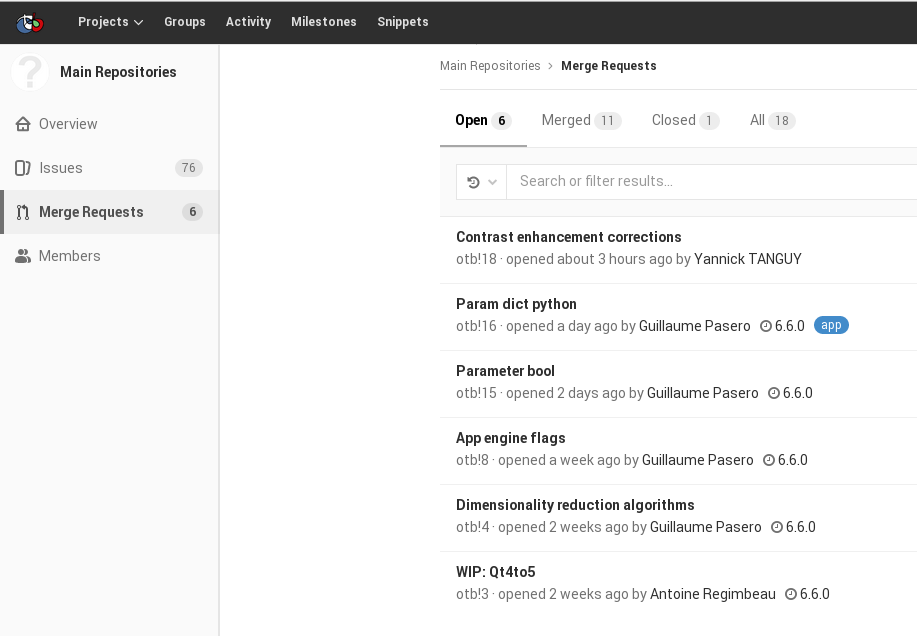
\includegraphics[width=\textwidth]{images/gitlab_mr.png}
    \end{columns}
\end{frame}
